\documentclass[a4paper, 11pt]{article}
\usepackage{covington}
\usepackage{amssymb}
\usepackage{amsmath}
\usepackage[catalan]{babel}
\usepackage{graphicx}
\usepackage{eurosym}
\usepackage{caption}
\usepackage{subcaption}
\usepackage{float}
\usepackage{bm}
\usepackage{layout}
\textheight=23.94cm 
\textwidth=17cm 
\topmargin=-1cm 
\oddsidemargin=-0.5cm 
 
\newcommand{\header}[4]{
	\begin{center}
		\rule{\linewidth}{0.5pt}
		
		{\small{#1}}
      
        \vspace{0.2in}
        
		{\large{#2}}
		
        \vspace{0.2in}
        
		{\small{#3}}
		
		\vspace{0.15in}
		
		{#4}
		
		\vspace{-0.1in}
		\rule{\linewidth}{0.6pt}
	\end{center}
}

\begin{document}
 
\header{\sc Barcelona Graduate School of Economics \hfill Master's Degree in Data Science}{\bf Statistical Modeling and Inference $-$ Problem Set \#4}{\sc Niti Mishra $\cdot$ Miquel Torrens $\cdot$ B\'alint V\'an}{November 9\textsuperscript{th}, 2015}
Solution to proposed exercises.\\
% EXERCISE 1
\newline \textbf{\underline{Exercise 1}}\\
\newline We need to show that $y(\mu + \sigma)$ is a point less than one standard deviation away from the mean of the marginal distribution of $t$, that is:
\begin{eqnarray}
y(\mu + \sigma) \leq \bar{t} + \sqrt{\mathbb{V}[t]} \nonumber
\end{eqnarray}
Given that $x \sim \mathcal{N}(\mu, \sigma^2)$ and $\varepsilon \sim \mathcal{N}(0, \tau^2)$ are assumed to be uncorrelated:
\begin{eqnarray}
\mathbb{E}[t] &=& \mathbb{E}[x + \varepsilon] = \mathbb{E}[x] + \mathbb{E}[\varepsilon] = \mu = \bar{t} \nonumber \\
\mathbb{V}[t] &=& \mathbb{V}[x + \varepsilon] = \mathbb{V}[x] + \mathbb{V}[\varepsilon] = \sigma^2 + \tau^2 \nonumber
\end{eqnarray}
We see that $\mu = \bar{t}$ because given the distribution of its components $t$ is a normally (and thus symmetrically) distributed around its mean, and has the same expected value as $x$. On the other hand:
\begin{eqnarray}
y(\mu + \sigma) = \mathbb{E}[t | x = \mu + \sigma] = \mu + \sigma \nonumber
\end{eqnarray}
And so we would need to show that:
\begin{eqnarray}
y(\mu + \sigma) &\leq& \mu + \sqrt{\mathbb{V}[t]} \nonumber \\
\mu + \sigma &\leq& \mu + \sqrt{\sigma^2 + \tau^2} \nonumber \\
\sigma^2 &\leq& \sigma^2 + \tau^2  \nonumber \\
\tau^2 &\geq& 0 \nonumber
\end{eqnarray}
We know that $\tau^2 \geq 0$ is indeed non-negative, thus proved.\\
% EXERCISE 2
\newpage
\textbf{\underline{Exercise 2}}\\
\newline \underline{Part (a)}\\
\newline We perform the following transformations to the raw data:
\begin{itemize}
\item Unify the fields \texttt{EARN1} and \texttt{EARN2} in one single field, adding an extra field named \texttt{INEXACT} that captures whether we use the precise answer from \texttt{EARN1} or the approximated answer in \texttt{EARN2}.
\item The resulting variable is called \texttt{EARNT} and is measured in thousands of dollars (e.g. \$10,000 has $\texttt{EARNT} = 10$).
\item Convert the field \texttt{HEIGHT} to total amount of inches and name it \texttt{HEIGHT\_I}.
\item Reescale the variable \texttt{SEX} to variable \texttt{MEN}, which takes value 1 if the individual is a man and 0 otherwise.
\item We suppress individuals with a reported weight greater than 500 (some have 990+ values for answer-codification reasons).
\item We suppress individuals with a reported height greater than 8 feet (some have 990+ values for answer-codification reasons).
\item We cut off the individual with highest income, as he reports an income that doubles the second highest income.
\end{itemize}
\underline{Part (b)}\\
\newline The regression run is the following:\\
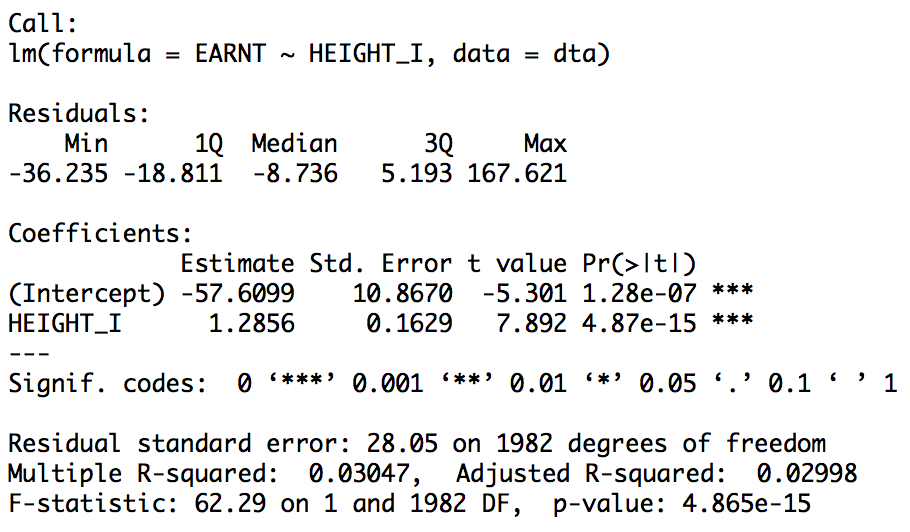
\includegraphics[scale=0.7]{reg1.png}
\newline The resulting parameter for \texttt{HEIGHT\_I} is imperceptibly sensitive to the inclusion of the control variable for exactness of income, although including it does boost the $R^2$ considerably and reduces the residual standard error.\\
\newline The transformation needed to interpret the intercept as average earnings for people with average height is substracting the mean fro the \texttt{HEIGHT\_I} variable. If we do so the resulting intercept is the following:\\
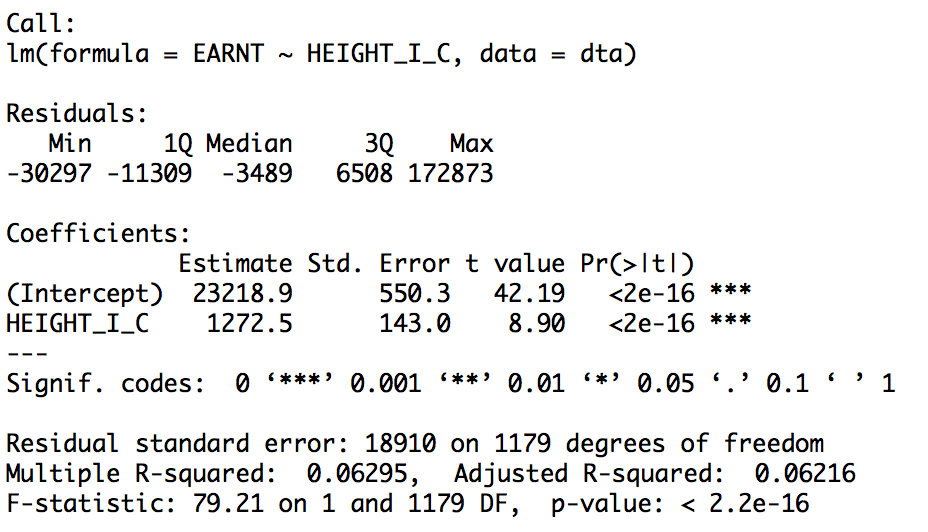
\includegraphics[scale=0.7]{reg2.png}
\newline This states that a person with average height will earn on average an income of  \$28,011 approximately.\\
\newline \underline{Part (c)}\\
\newline We have run the following models:\\
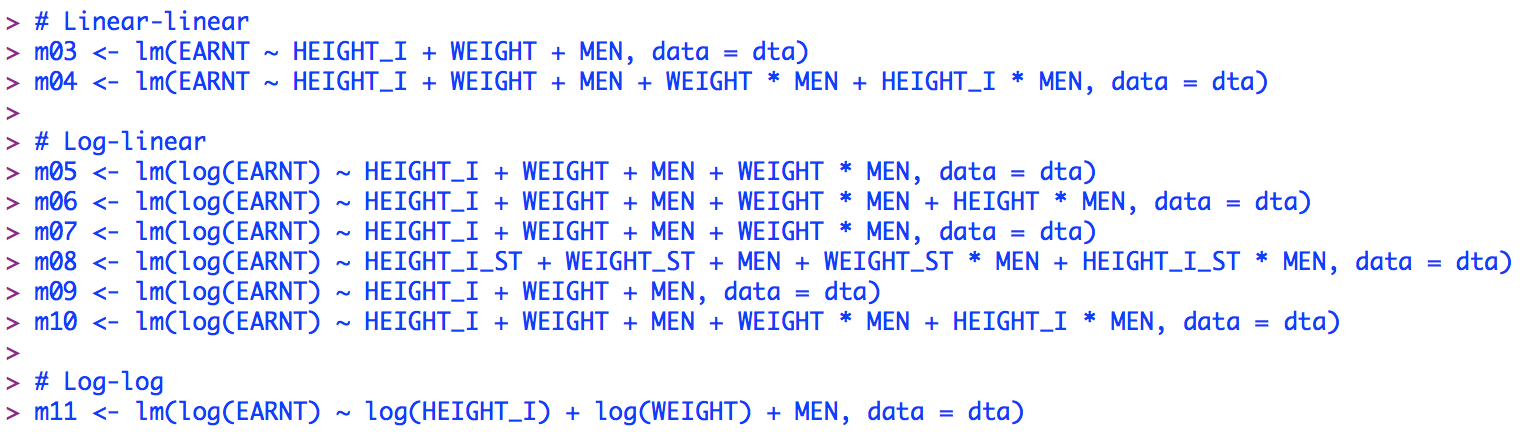
\includegraphics[scale=0.5]{reg3.png}
\newline In the models that use logarithms we only use the observations with positive earnings.\\
\newline We choose model \texttt{m13} for several reasons. First, the residual standard error is the smallest between within log-linear models; second, it has a relatively high $R^2$ and, third, the regressors are all significant and have an intuitive sign. The results are the following:\\
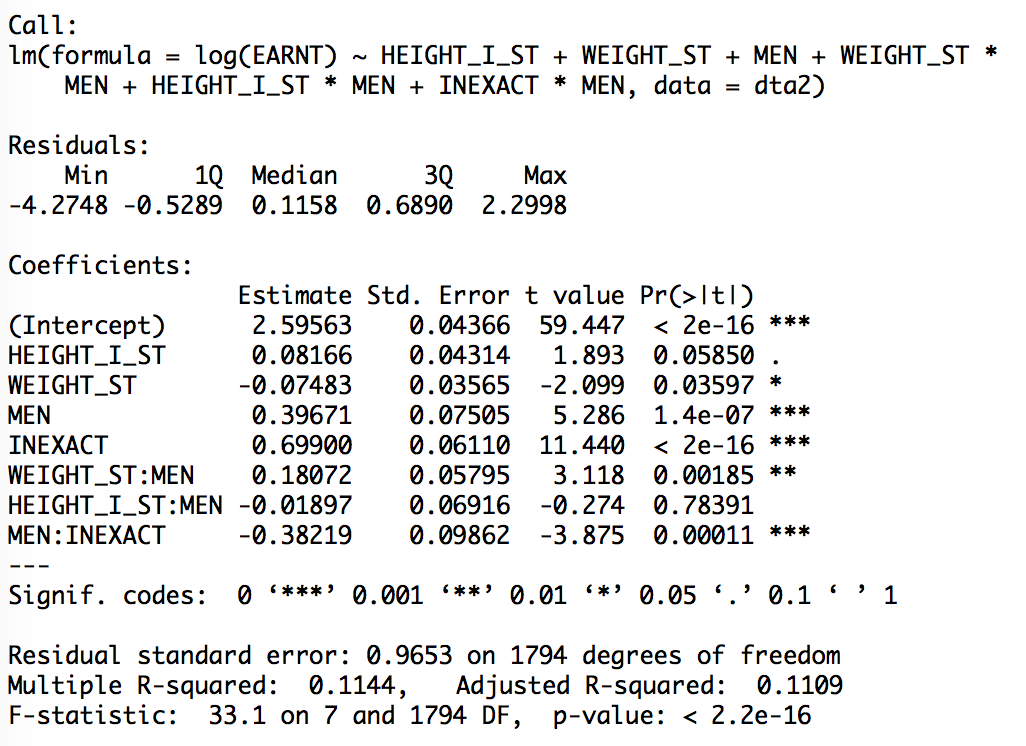
\includegraphics[scale=0.7]{reg4.png}
\newline \\
\newline \underline{Part (d)}\\
\newline The results are only for strictly positive income individuals. The interpretation of the coefficients is the following:
\begin{itemize}
\item The intercept says that a woman of average height and weight (who would report the exact amount of salary) is expected to earn $1,000 \times \exp{(2.5956)} = \$13,405$.
\item The coefficient for \texttt{HEIGHT\_I\_ST} says that exceeding the average height by one standard deviation increases the expected income by 8.1\%. Exceeding by two standard deviations would increase the expected salary by 16.2\%, and so on. In the case of men, this is diminished by the coefficient of \texttt{HEIGHT\_I\_ST:MEN}, which sets the total increase for men to 5.7\% when one standard deviation away, although this coefficient is not significant.
\item The coefficient for \texttt{WEIGHT\_ST} says that exceeding the average weight by one standard deviation decreases the expected income by 7.6\%. In the case of men, this is actually overturned by the coefficient on \texttt{WEIGHT\_ST:MEN}, and the aggregated effect is of +10.9\% on income, so the data shows a negative effect on women and positive on men.
\item The coefficient on \texttt{MEN} suggests that an man of average height and weight earns on average 27.3\% more than a woman of average height and weight.
\item The coefficient on \texttt{INEXACT} means that a woman who reports inexact answers is expected to earn 69.9\% more. In the case of men, we add the value of the interaction term to expect an increase of 31.7\% for the average man.
\end{itemize}
% EXERCISE 3
\newpage
\textbf{\underline{Exercise 3}}\\
\newline \underline{Part (a)}\\
\newline We generate random draws and plot the result:
\begin{center}
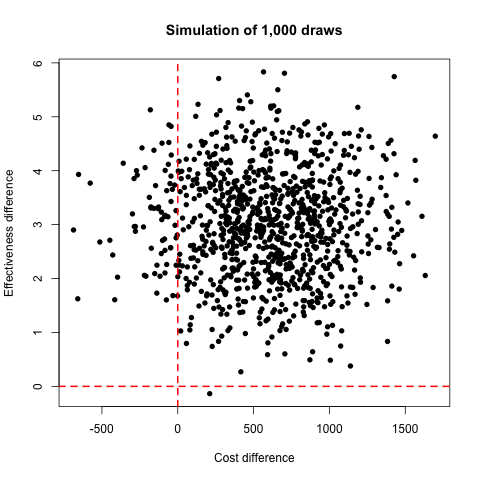
\includegraphics[scale=0.6]{plot_ex3dot1.png}
\end{center}
\underline{Part (b)}\\
\newline We take the sample ratio of the simulations we have drawn. We take the quantile of this sample ratio and keep the corresponding quantiles.\\
\newline For the 50\% case, we take quantiles 25\% and 75\%, leaving 50\% of the sample inside (50\% confidence interval). The interval is $(108.7, 313.7)$\\
\newline For the 50\% case, we take quantiles 2.5\% and 97.5\%, leaving 95\% of the sample inside (95\% confidence interval). The interval is $(-57.3, 677.9)$.\\
\newline \underline{Part (b)}\\
\newline The plot is the following:
\begin{center}
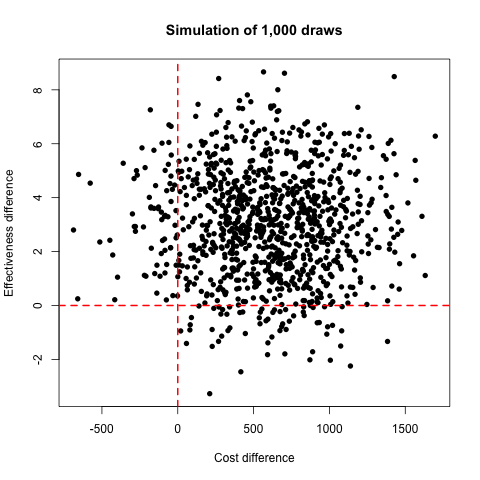
\includegraphics[scale=0.6]{plot_ex3dot3.png}
\end{center}
The intervals in this case are the following:
\begin{itemize}
\item 50\% confidence interval: $(71.2, 326.9)$.
\item 95\% confidence interval: $(-1386.8, 2122.8)$.
\end{itemize}
% EXERCISE 4
\newpage
\textbf{\underline{Exercise 4}}\\
\newline We plot a histogram the district share of democratic votes data for 1988:
\begin{center}
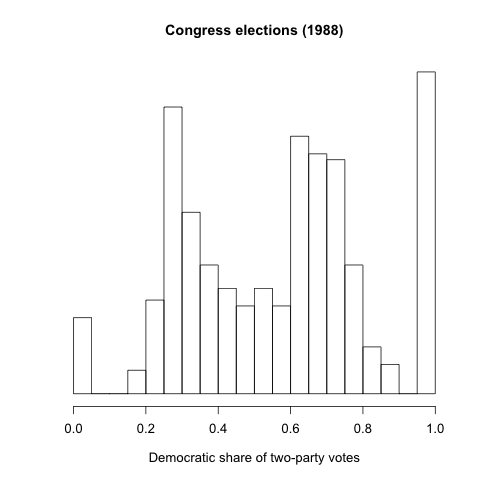
\includegraphics[scale=0.5]{plot_ex4_1.png}
\end{center}
Districts with less than 10\% share are condensed towards zero and districts with more than 90\% are condensed towards one, as they represent uncontested districts.\\
\newline We will try to run a linear regression model that predicts the democratic share of vote in 1988 given the share of vote from the previous election and the sign of the party of the incumbent until the election.
\begin{figure}[H]
\centering
\begin{subfigure}{.5\textwidth}
  \centering
  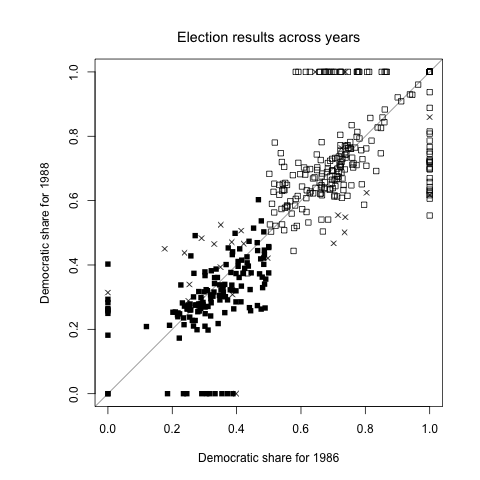
\includegraphics[width=1\linewidth]{plot_ex4_2.png}
\end{subfigure}%
\begin{subfigure}{.5\textwidth}
  \centering
  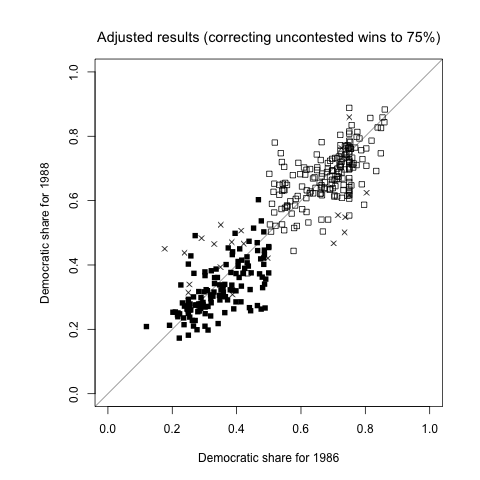
\includegraphics[width=1\linewidth]{plot_ex4_3.png}
\end{subfigure}
\end{figure}
In the first plot, bolded squares are districts with Republican incumbents in 1988, white squares belong to Democratic incumbents and crosses represent open seats. The line represented is the 45 degree line. In the second plot we show the same picture but correcting for uncontested wins in 1986, adjusting the shares to 75\%-25\% in favor of the 1986 uncontested winner.\\
\newline The regression is run using only the contested wins in 1988 using the adjusted data. The incumbent variable is coded as follows: $-1$ for Republican holder, $1$ for Democratic holder and $0$ for open seat. The summary of the model is the following:\\
\newline \\
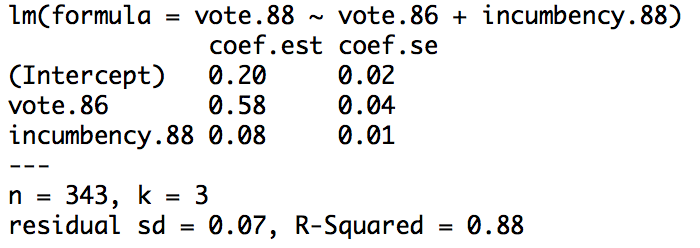
\includegraphics[scale=0.7]{plot_ex4_4.png}
\newline \\
\newline Now, with these results we would like to estimate the outcome for the following election in 1990. To do this, we use 1,000 predictive simulations drawn with the book's \texttt{sim()} function. We multiply the new data (share of votes of 1988 and incumbent as of 1990) and we multiply it with the coefficients of the predictive simulations (that is, $\mathbf{\Phi}_{90} \mathbf{w}$) and we add normally distributed errors.\\
\newline The results of this simulations show for each district (total of 435) what will the Democratic share of votes be for each simulation (total of 1,000), thatt is, a $1000 \times 435$ matrix. The districts won uncontested in 1990 have values \texttt{NA} as the model does not predict them. We set these to zero.\\
\newline The number of elections won by the Democrats in 1990 is predicted using the simple rule of win in case the predicted value is above 50\% and lose otherwise. The results are shown in the book's Figure 7.5, which we approximately replicate here:
\begin{center}
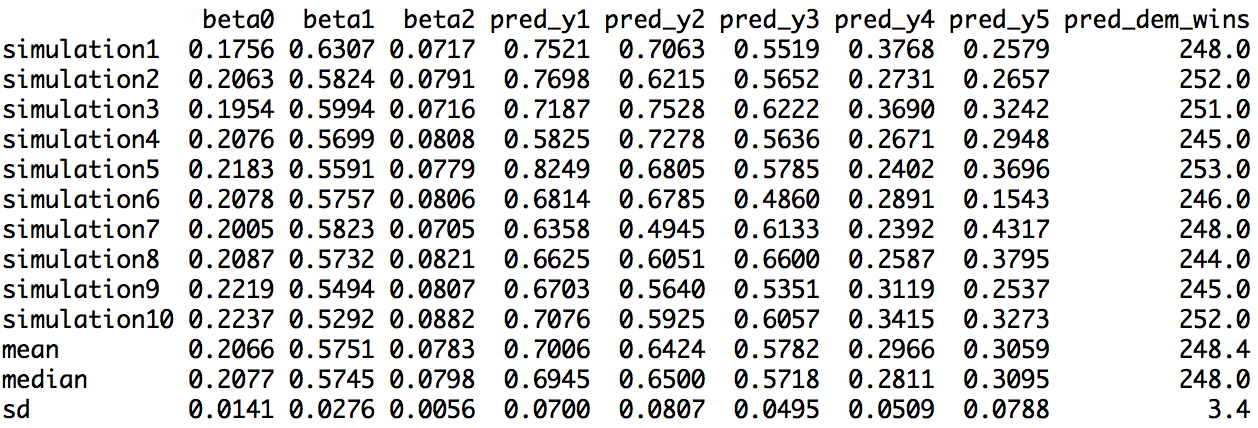
\includegraphics[scale=0.7]{plot_ex4_5.png}
\end{center}
Gelman and Hill show that the average total wins predicted was actually way off the final result, which was 260, more than three standard deviations away from the mean, so this model does not really look applicable to 1990.
\end{document}





